\newpage
\section{Lexical Analysis}
To translate a program from one language into another, a compiler first pull it apart and understand its structure and meaning, then put it together in a different way.

\begin{itemize}
    \item The front end(前端): performs analysis
    \item The back end(后端): performs synthesis
\end{itemize}

The analysis is usually broken up into:
\begin{enumerate}
    \item Lexical analysis
    \item Syntax analysis
    \item Semantic analysis
\end{enumerate}

% Task of the lexical analyzer:

\subsection{Lexical Token}
\subsubsection{A lexical token}
\begin{itemize}
    \item A sequence of characters
    \item A unit in the grammar of a programming language
\end{itemize}

\subsubsection{Token types}
Classification of lexical tokens: A finite set of token types.

e.g.
\begin{itemize}
    \item %TODO
\end{itemize}


\subsubsection{Non-Tokens}
e.g.
\begin{itemize}
    \item %TODO
\end{itemize}

\subsubsection{An example}
\begin{minted}{c}
float match0(char *s){ /* find a zero */
    if (!strncmp(s, "0.0", 3))
        return 0.;
}
\end{minted}

\begin{minted}{text}
FLOAT ID(match0) LPAREN CHAR STAR ID(s) RPAREN LBRACE 
IF LPAREN BANG ID(strncmp) LPAREN ID(s) COMMA STRING(0.0) COMMA NUM(3) RPAREN RPAREN 
RETURN REAL(0.0) SEMI 
RBRACE EOF
\end{minted}



\subsubsection{An ad hoc lexer}
Any reasonable programming language can be used to implement it

\subsubsection{A simpler and more readable lexical analyzers}
\begin{itemize}
    \item Regular expressions :Specify lexical tokens
    \item Deterministic finite automata : Implementing lexers
    \item Mathematics: Connecting the above two
\end{itemize}

\subsection{Regular Expression}
\subsubsection{Some Concepts}
\begin{itemize}
    \item A language is a set of strings
    \item A string is a finite sequence of symbols
    \item A symbol is taken from a finite alphabet
\end{itemize}

\subsubsection{The notation of regular expressions}
\begin{itemize}
    \item Symbol: a
    \item Alternation: A vertical bar $||$
    \item Concatenation: operator $\cdot$
    \item Epsilon: $\epsilon$
    \item Repetition: ${}^*$
    \subitem Given a regular expression $M$, its Kleene closure is $M^*$.
    \subitem A string is in $M^*$ if it is the concatenation of zero or more strings, all of which are in M.
\end{itemize}

优先级: ${}^*> \cdot > ||$.

\begin{figure}[!htb]
    \centering
    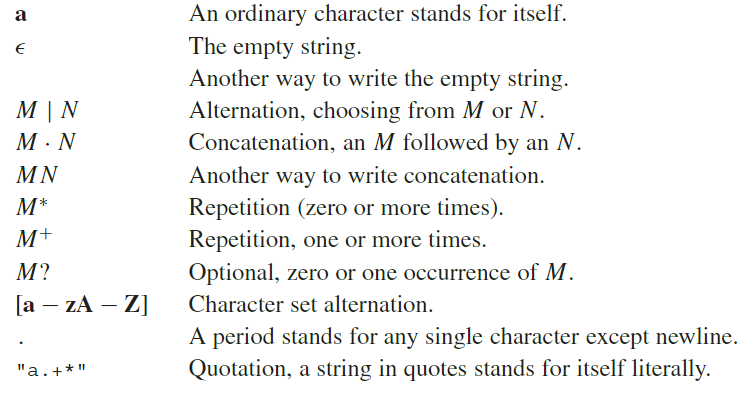
\includegraphics[width=0.42\textwidth]{pic/CP2/Regular expression notation}
    \caption{Regular expression notation}
\end{figure}

\begin{figure}[!htb]
    \centering
    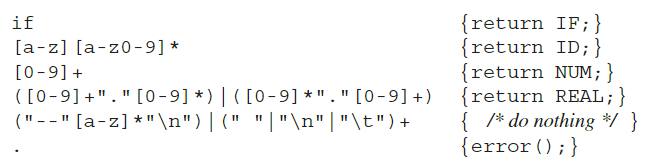
\includegraphics[width=0.42\textwidth]{pic/CP2/Regular expressions for some tokens}
    \caption{Regular expressions for some tokens}
\end{figure}

\subsubsection{Two important disambiguation rules}
These rules are a bit ambiguous.

\begin{enumerate}
    \item Longest match
    \subitem The longest initial substring of the input that can match any regular expression is taken as the next token.
    \item Rule priority
    \subitem The first regular expression that can match determines its token-type
\end{enumerate}